\documentclass{article}
\usepackage[utf8]{inputenc}
\usepackage[greek,english]{babel}
\usepackage{alphabeta}
\usepackage{fancyhdr}
\usepackage{listings}
\usepackage{mathtools}
\usepackage{xcolor}
\usepackage{graphicx}
\usepackage{float}
\usepackage[backend=biber]{biblatex}

\title{Σήματα και Συστήματα - Εργασία 4}
\author{Χρήστος Μαργιώλης - 19390133}
\date{Μάιος 2021}

\begin{document}

\begin{titlepage}
        \maketitle
        \begin{figure}[t!]
        \begin{center}
        
\includegraphics[scale=0.3]{./res/uniwalogo.png} \\
        \Large
        \textbf{Πανεπιστήμιο Δυτικής Αττικής} \\
        \large
        Τμήμα Μηχανικών Πληροφορικής και Ηλεκτρονικών Υπολογιστών
        \end{center}
        \end{figure}
\end{titlepage}

\renewcommand{\contentsname}{Περιεχόμενα}
\tableofcontents

\section{'Ασκηση 1}

\begin{itemize}
	\item Σε σύστημα με κορυστική απόκριση $h(t) = t, 0 \leq t \leq 10$
		έχουμε είσοδο $x(t) = 0.8^t, 0 \leq t \leq 10$. Ζητείται να
		σχεδιάσετε την έξοδο του συστήματος.
\end{itemize}

Αρχικά θα ορίσουμε την απόκριση $h(t)$ και την είσοδο $x(t)$ στο διάστημα
$0 \leq t \leq 10$:

\begin{lstlisting}[language=octave]
	octave> t = 0:.01:10
	octave> h = t
	octave> x = 0.8.^t
\end{lstlisting}

Για τον υπολογισμό της συνέλιξης χρησιμοποιούμε την συνάρτηση \lstinline{conv()}
και θα την πολλαπλασιάσουμε με 0.01 ώστε να προσσεγίσουμε το ολοκλήρωμα από
άθροισμα:

\begin{lstlisting}[language=octave]
	octave> y = conv(x,h)*0.01
\end{lstlisting}

Προκειμένου να φαίνεται σωστά η γραφική παράσταση, θα ορίσουμε τον άξονα $x$
από 0 εως το 20:

\begin{lstlisting}[language=octave]
	octave> tx = 0:.01:20
	octave> plot(tx,y)
\end{lstlisting}

\begin{figure}[H]
        \centering
        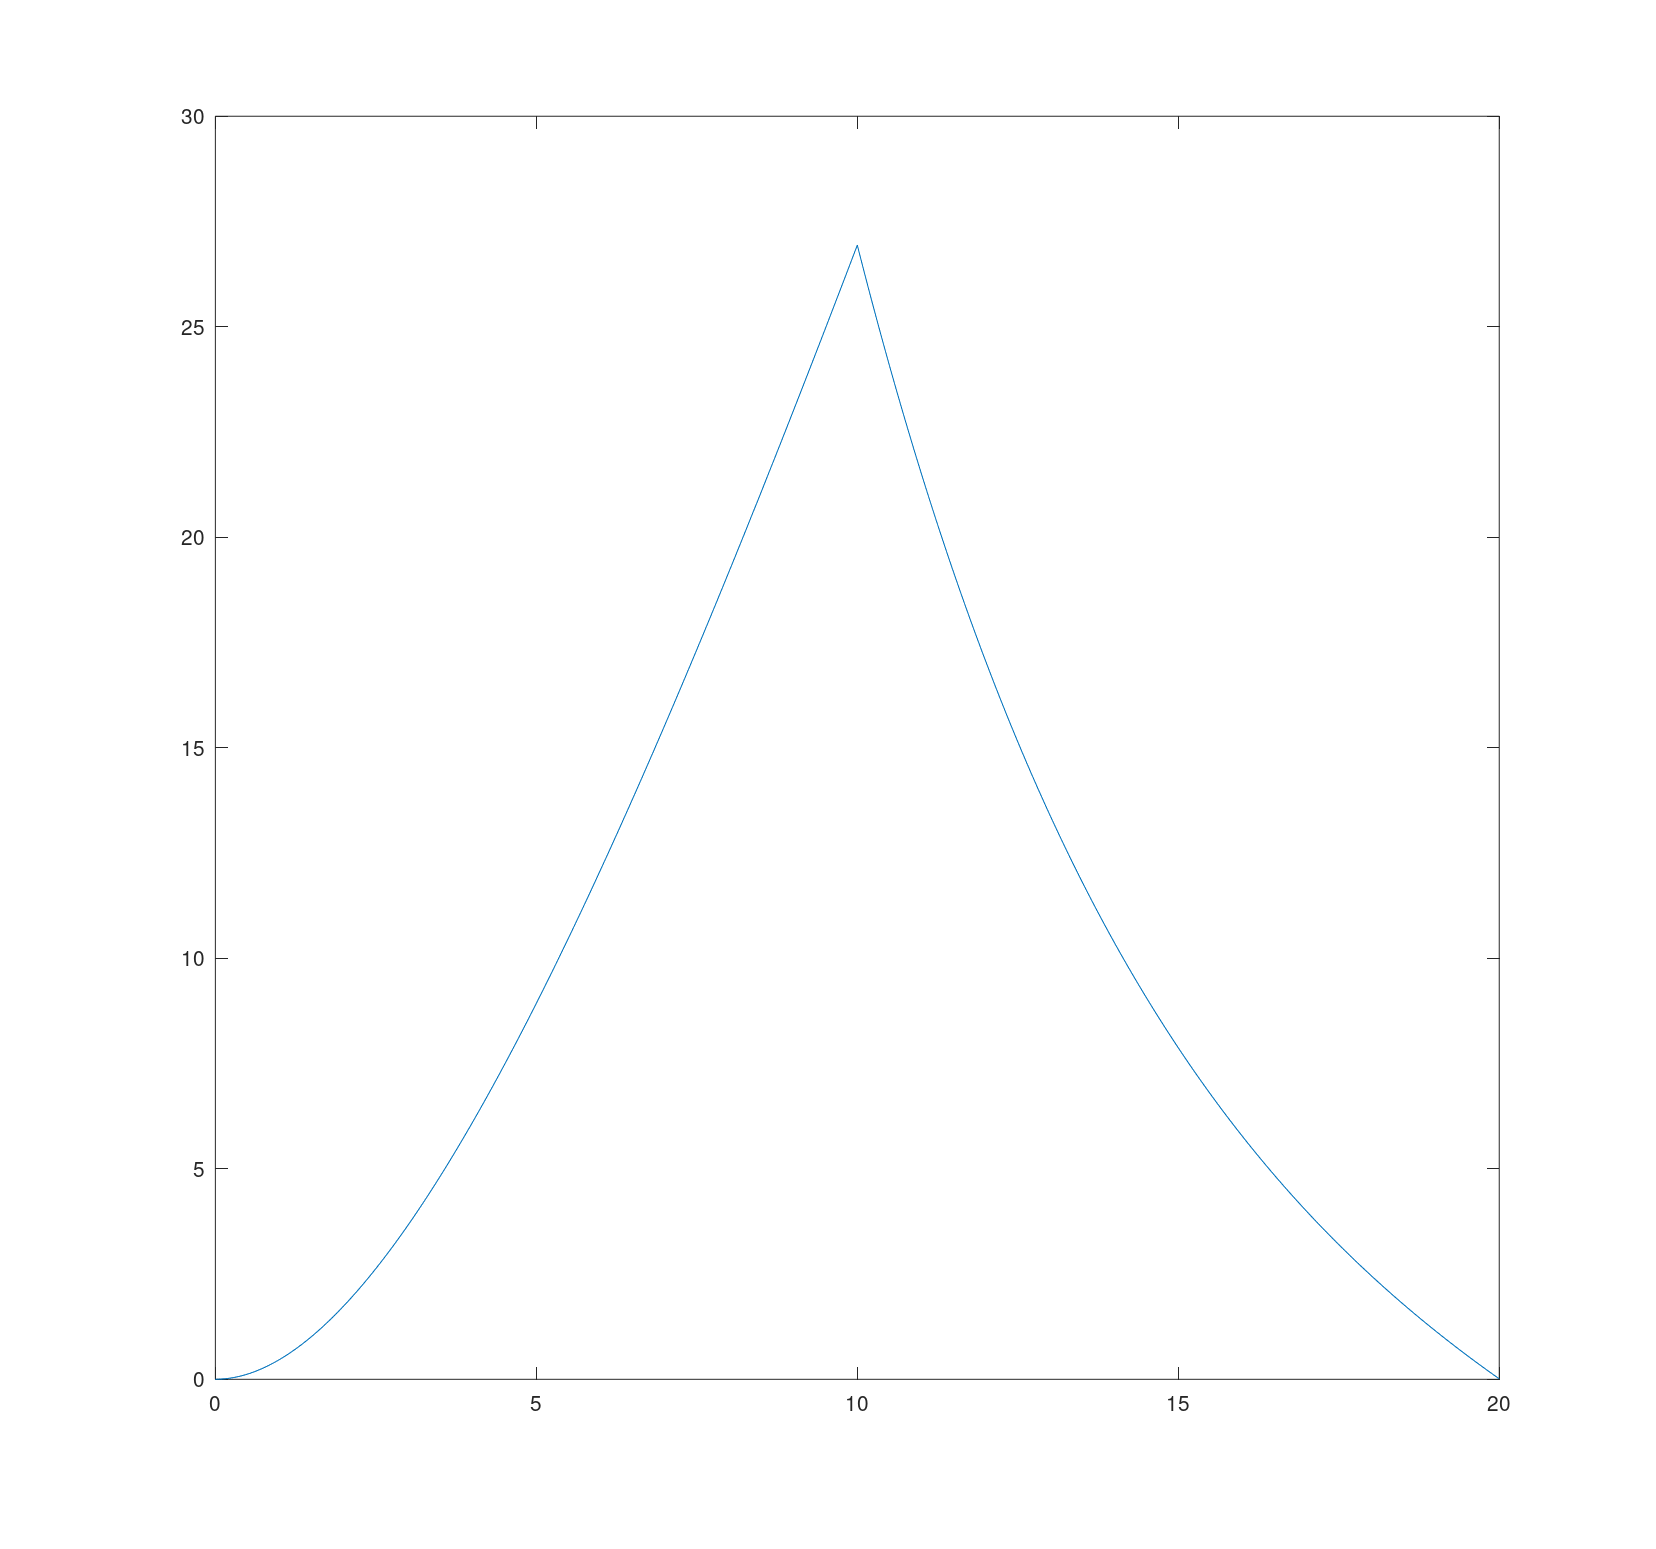
\includegraphics[width=\linewidth]{res/fig1.png}
\end{figure}

\section{'Ασκηση 2}

\begin{itemize}
	\item Σε σύστημα με κρουστική απόκριση $h(t) = e^{-2t}u(t - 1)$ έχουμε
		είσοδο $x(t) = u(t) - u(t - 2)$. Ζητείται να σχεδιάσετε
		την έξοδο.
\end{itemize}

Με παρόμοιο τρόπο όπως και στην άσκηση 1 θα υπολογίσουμε και την έξοδο
του $h(t)$. Η μόνη διαφορά είναι ότι για να υπολογίστουνε τα $u(t)$
θα χρειαστεί η συνάρτηση \lstinline{heaviside()}.

\begin{lstlisting}[language=octave]
	octave> t = 0:.01:10
	octave> h = exp(-2*t).*heaviside(t-1)
	octave> x = heaviside(t)-heaviside(t-2)
	octave> y = conv(x,h)*0.01
	octave> tx = 0:.01:20
	octave> plot(tx, y)
\end{lstlisting}

\begin{figure}[H]
	\centering
	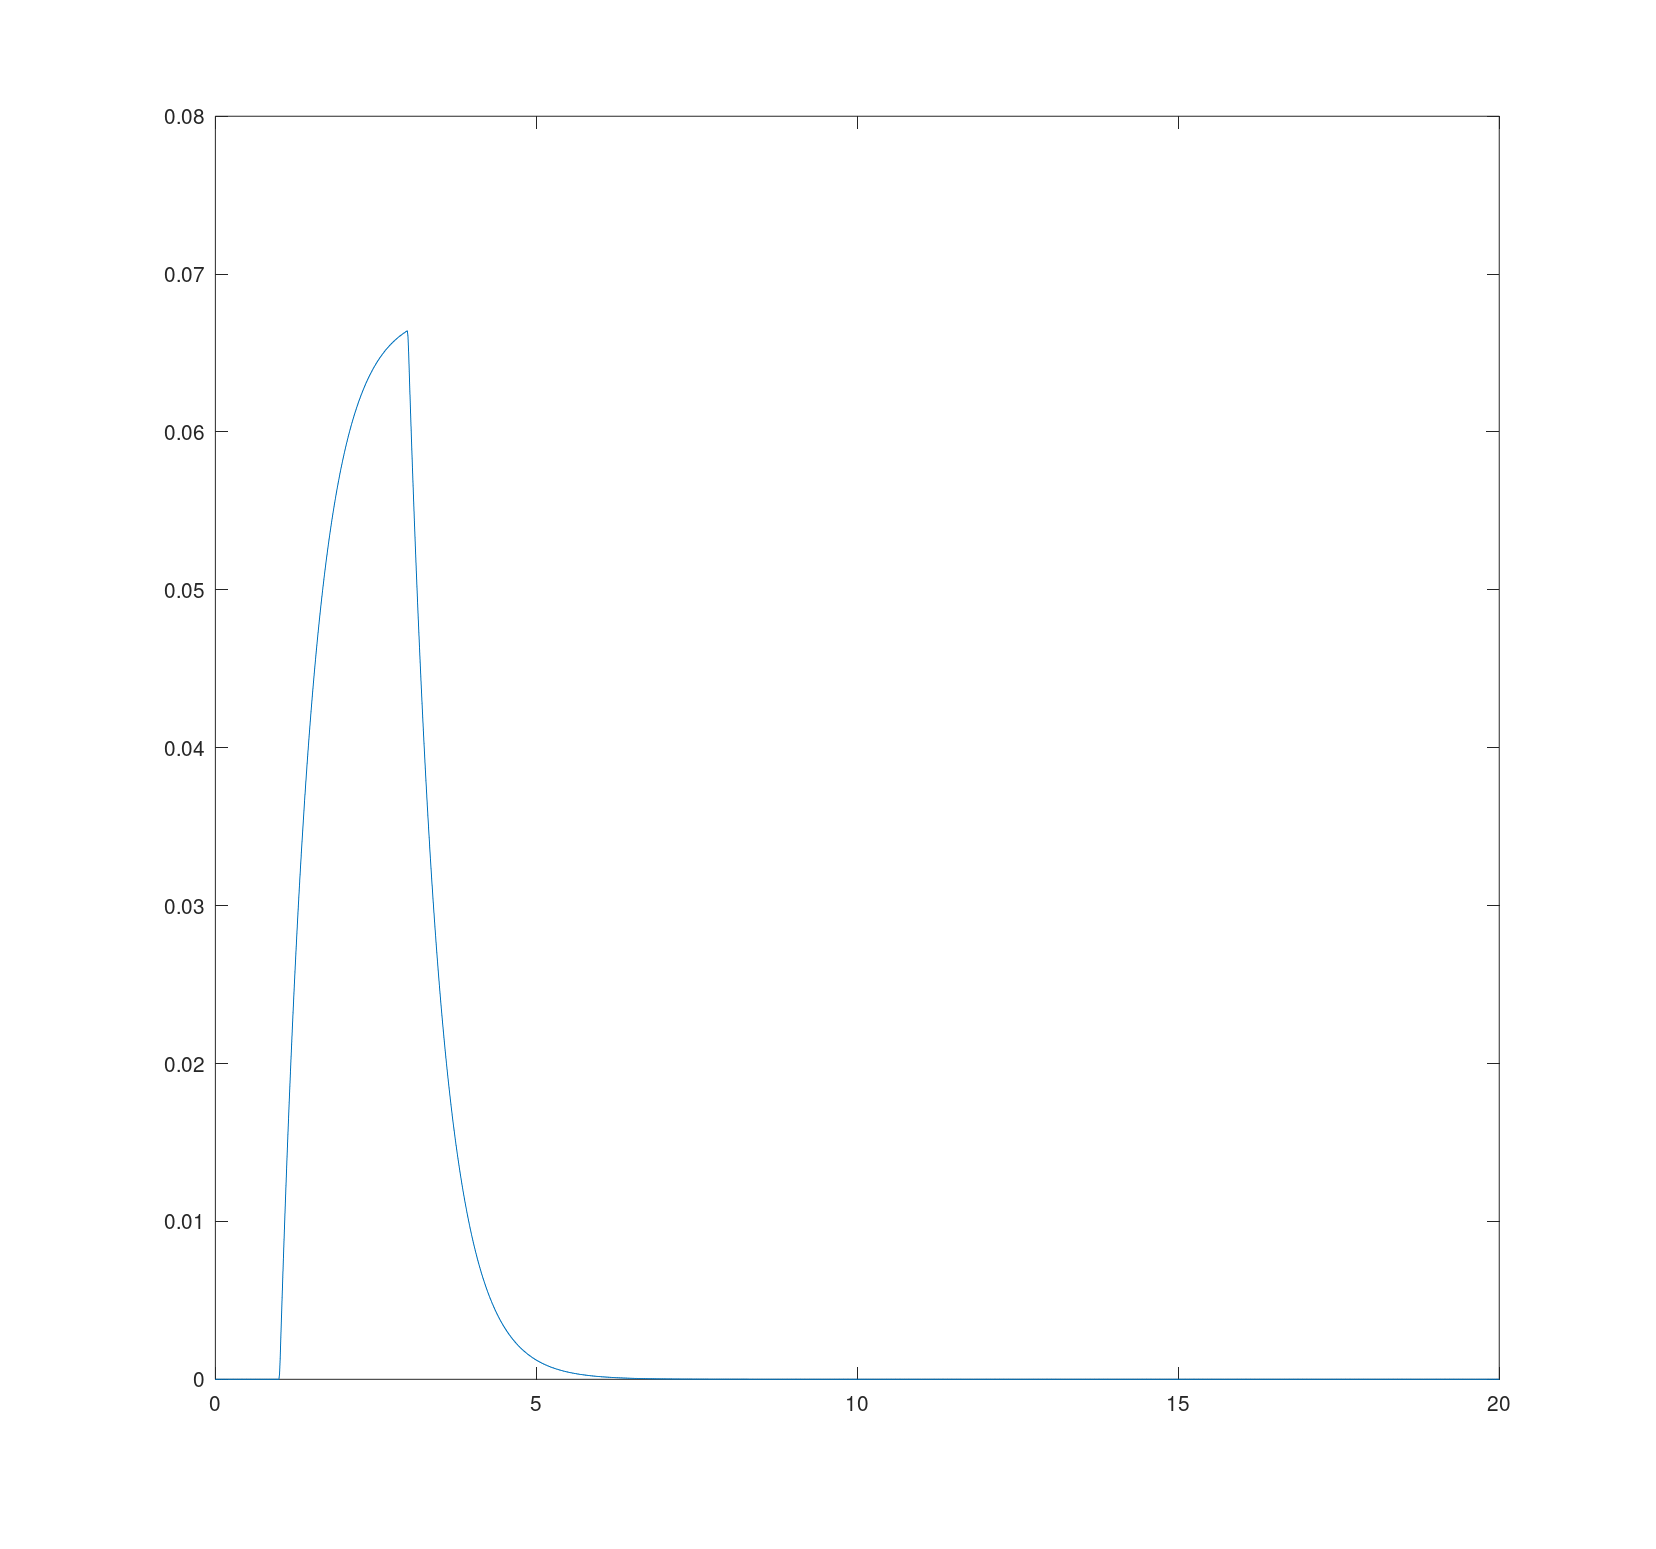
\includegraphics[width=\linewidth]{res/fig2.png}
\end{figure}

\section{'Ασκηση 3}

\begin{itemize}
        \item Θεωρείστε το Γ.Χ.Α σύστημα με κρουστική απόκριση
		$h(t) = e^{-3t}u(t)$. Υπολογίστε και σχεδιάσετε την
		απόκριση (έξοδο) του συστήματος στην είσοδο
		$x(t) = u(t + 2) - u(t - 3)$.
\end{itemize}

\begin{lstlisting}[language=octave]
	octave> t = -2:.1:10
	octave> h = exp(-3*t).*heaviside(t)
	octave> x = heaviside(t+2)-heaviside(t-3)
	octave> y = conv(x,h)*.1
	octave> tx = -4:.1:20
	octave> plot(tx, y)
\end{lstlisting}

\begin{figure}[H]
	\centering
	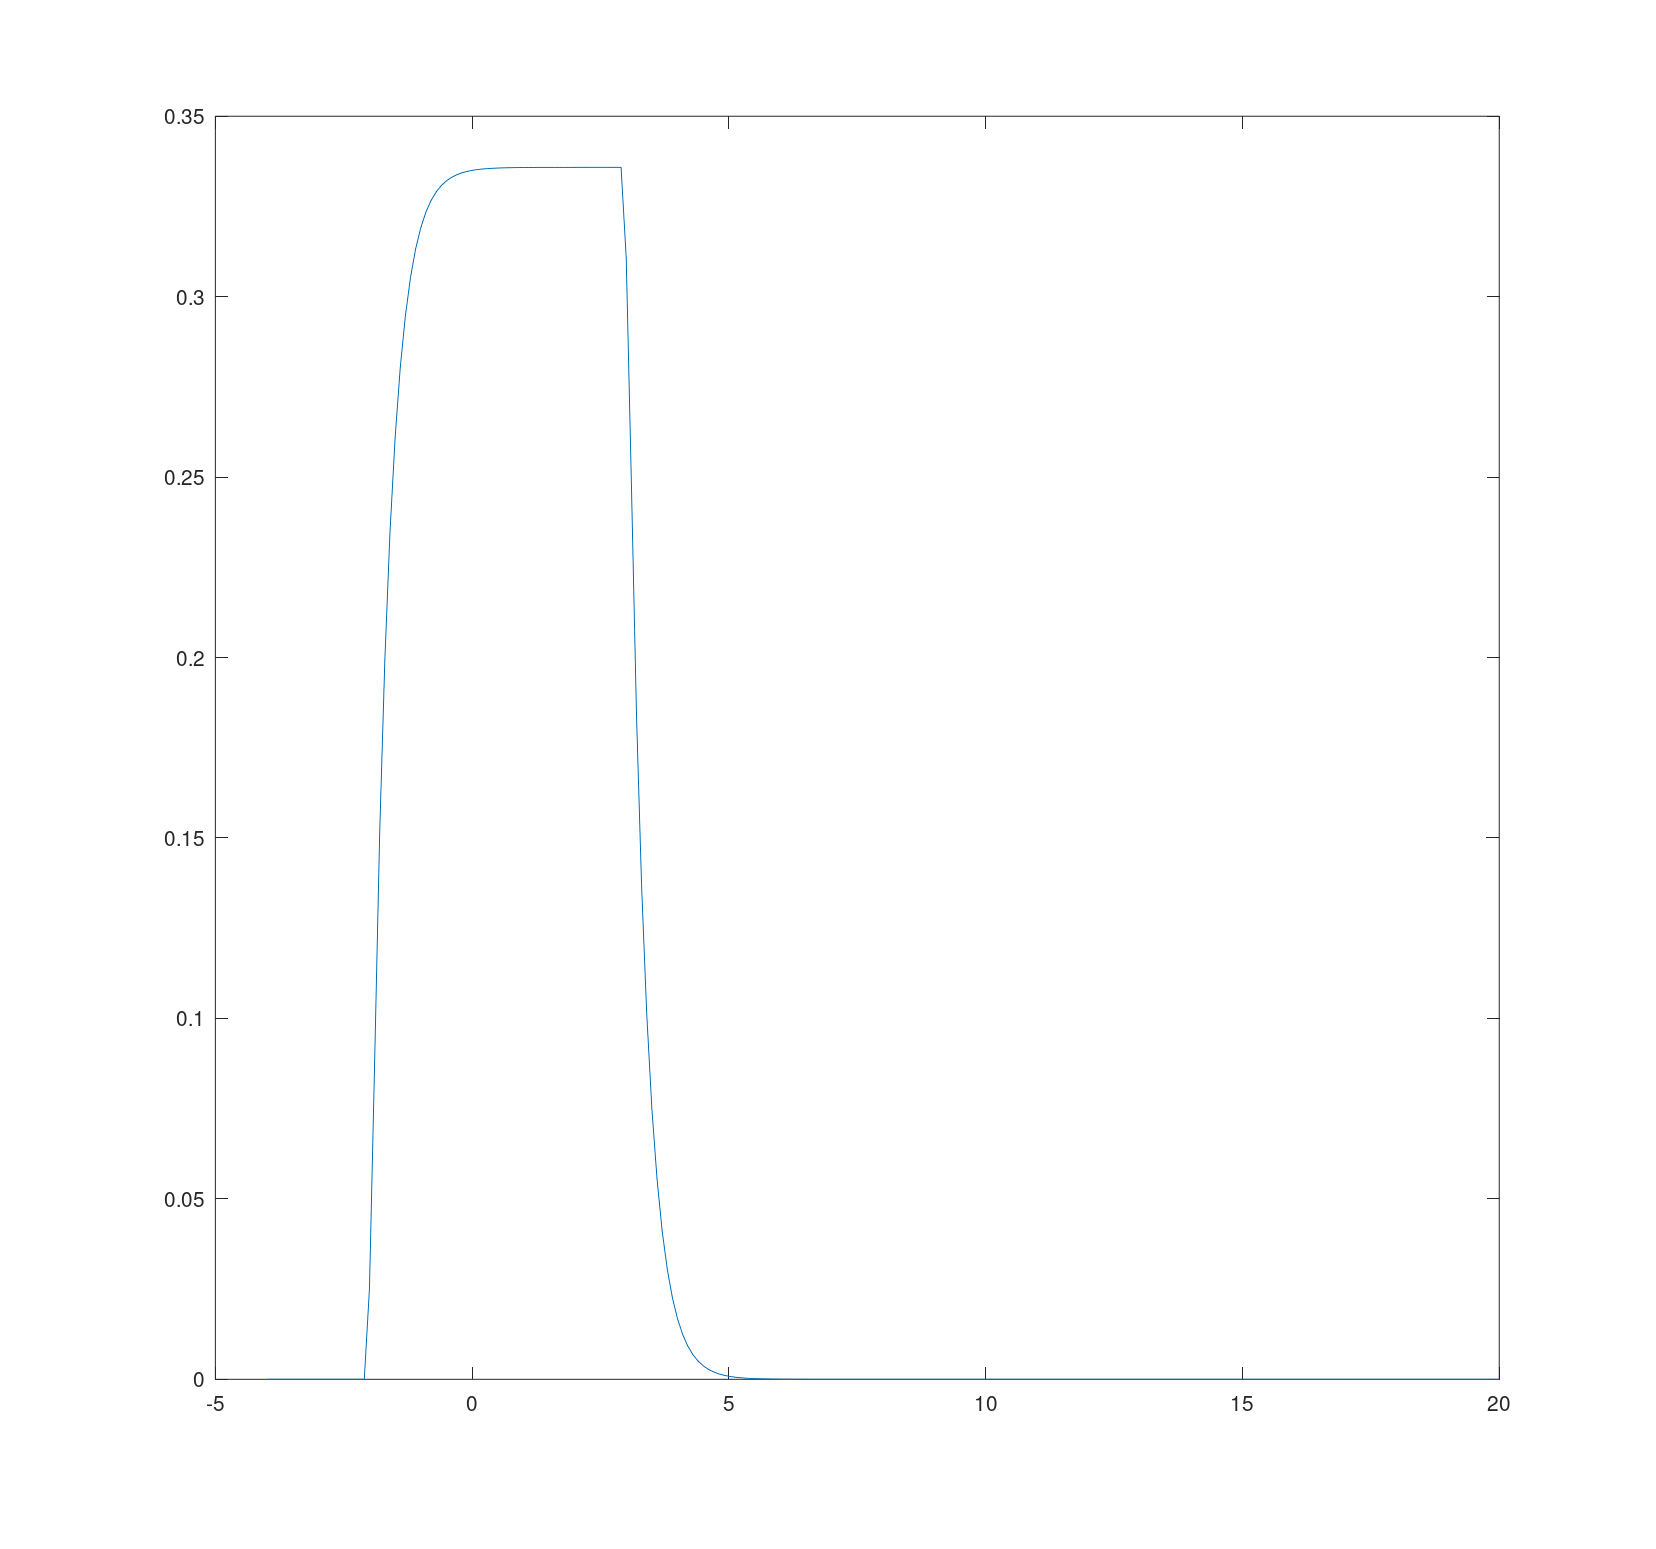
\includegraphics[width=\linewidth]{res/fig3.png}
\end{figure}

\section{'Ασκηση 4}

\begin{itemize}
        \item Σχεδιάστε το αποτέλεσμα της συνέλιξης των σημάτων που φαίνονται
		στο σχήμα (φυλ. εργασίας σελ. 18).
\end{itemize}

\begin{lstlisting}[language=octave]
	octave> t1 = 0:.01:2
	octave> t2 = 2.01:.01:4
	octave> t3 = 4.01:.01:5
	octave> x1 = zeros(size(t1))
	octave> x2 = ones(size(t2))
	octave> x3 = zeros(size(t3))
	octave> x = [x1 x2 x3]
	octave> h1 = ones(size(t1))
	octave> h2 = zeros(size([t2 t3]))
	octave> h = [h1 h2]
	octave> y = conv(x,h)*.01
	octave> tx = 0:.01:10
	octave> plot(tx, y)
\end{lstlisting}

\begin{figure}[H]
	\centering
	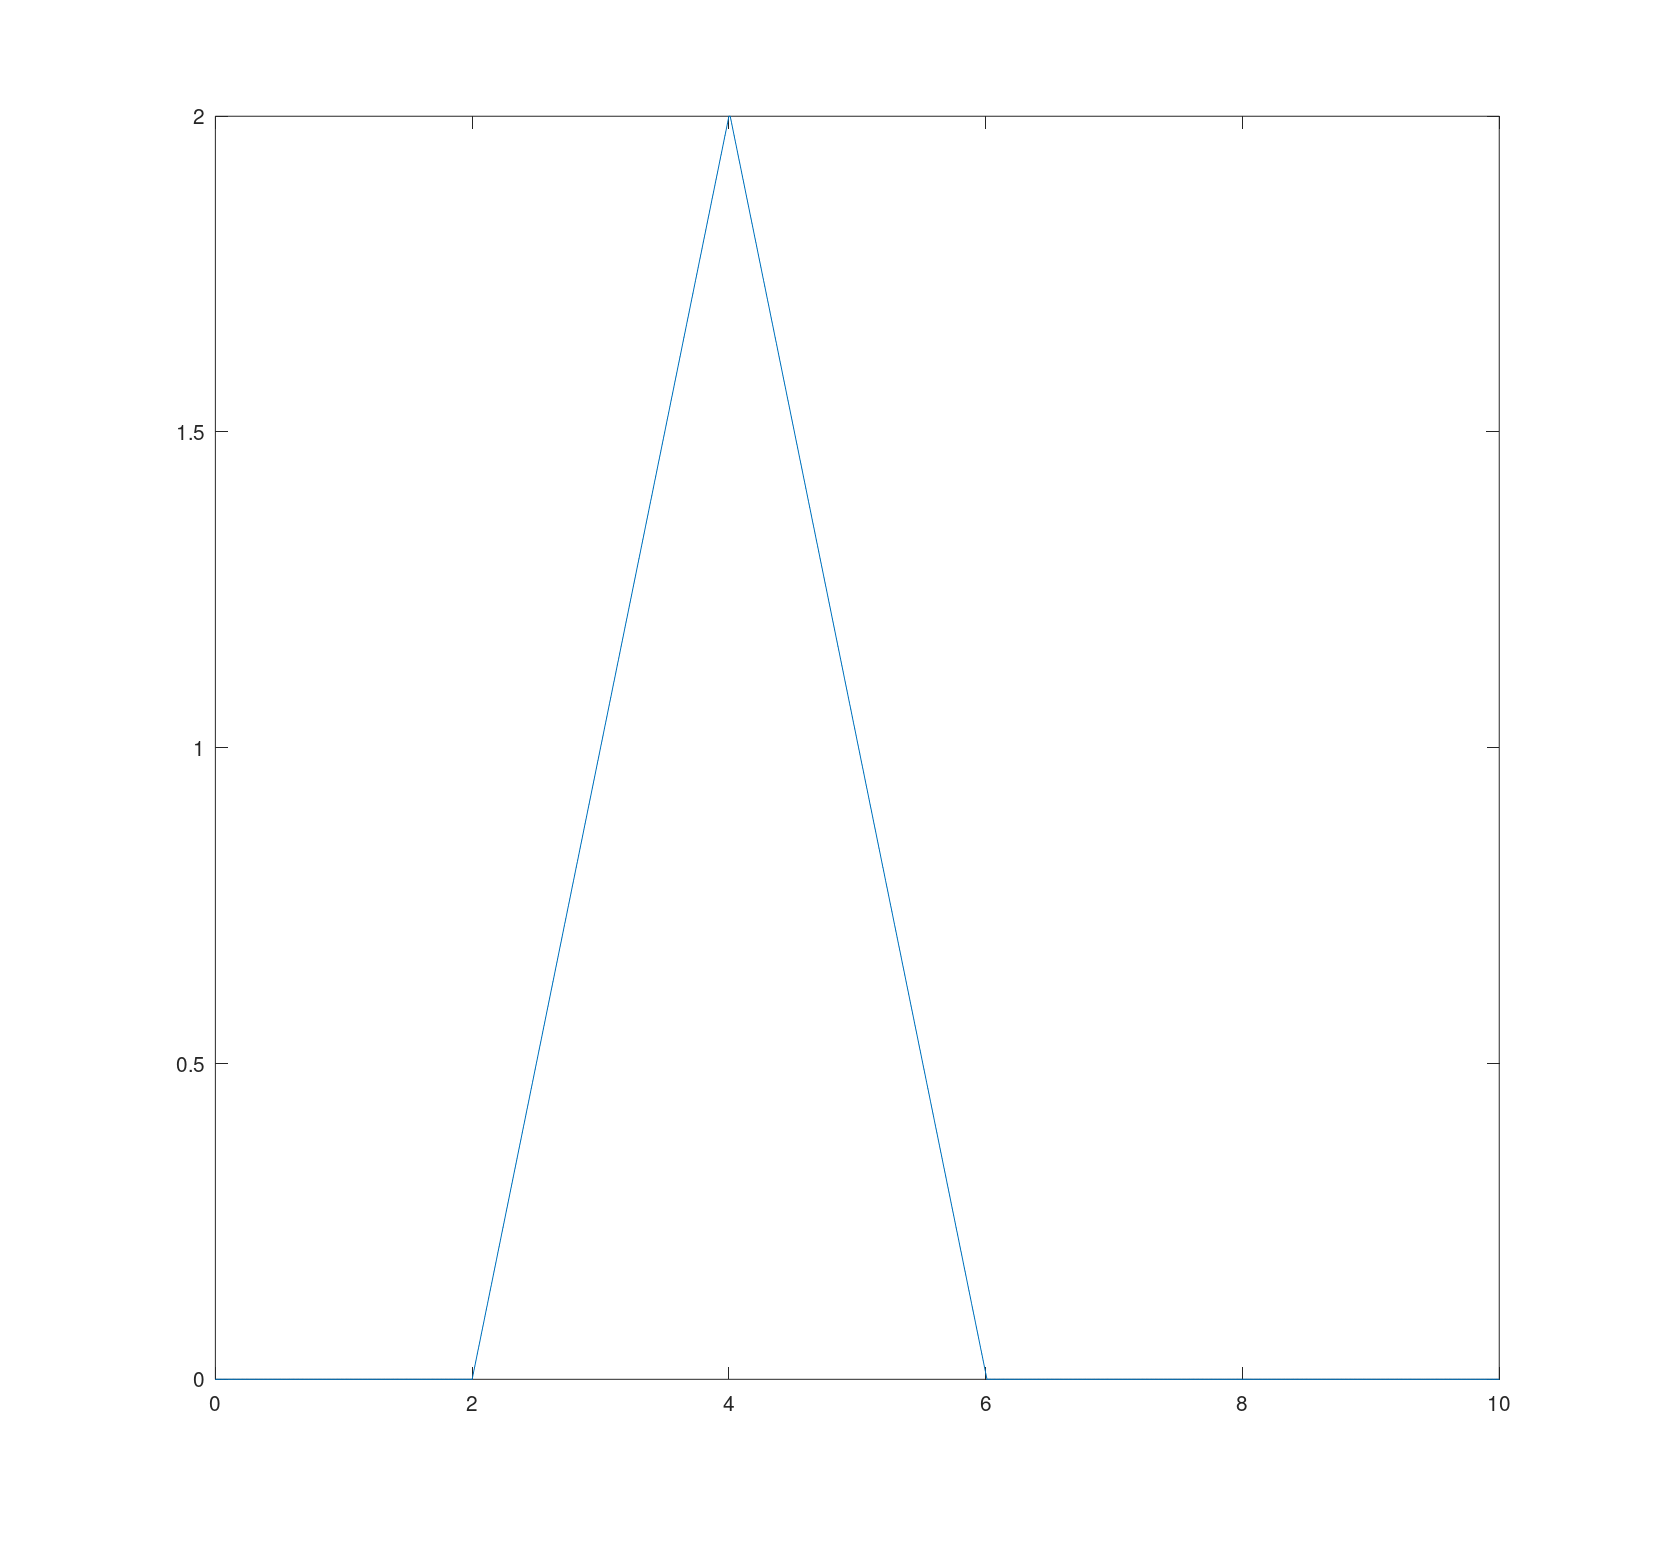
\includegraphics[width=\linewidth]{res/fig4.png}
\end{figure}

\section{'Ασκηση 5}

\begin{itemize}
	\item Δίνεται σύστημα με κρουστική απόκριση $h(t) = te^{-t}u(t)$. Να
		σχεδιαστεί η έξοδος του συστήματος για την είσοδο $x(t)$
		του σχήματος (φυλ. εργασίας σελ 18).
\end{itemize}

Δεν έγινε.

\section{'Ασκηση 6}

\begin{itemize}
        \item Έστω γραμμικό χρονικά αναλλοίωτο σύστημα που έχει κρουστική
		απόκριση
		\[
			h(t) = 
			\left\{
				\begin{array}{ll}
				1-t  & 0 \leq t \leq 1 \\
				-x & \mbox{αλλού}
			\end{array}
			\right.
		\]
		Υπολογίστε την απόκρισή του
		\begin{itemize}
			\item Αναλυτικά, κάνοντας και τη γραφική παράσταση
				των σημάτων $x$ και $h$ στα διάφορα στάδια του
				υπολογισμού του ολοκληρώματος.
			\item Προσεγγιστικά, με τη βοήθεια της συνέλιξης
				διακριτού χρόνου (\lstinline{conv}).
		\end{itemize}
\end{itemize}

Δεν έγινε.

\pagebreak
\section{Εργαλεία}
Τα εργαλεία που χρησιμοποιήθηκαν για την υλοποίηση αυτής της εργασίας ήτανε
τα εξής:
\begin{itemize}
        \item Περιβάλλον: GNU Octave 6.2.0
        \item Επιπλέον πακέτα:
        \begin{itemize}
                \item \lstinline{octave-forge-symbolic}
                \item \lstinline{octave-forge-signal}
        \end{itemize}
        \item Λειτουργικό σύστημα: FreeBSD 12.2
        \item Κειμενογράφος: Vim
        \item Μορφοποίηση κειμένου: \LaTeX
\end{itemize}

\end{document}
